\chapter{Introduction}
\section{Water Cycle}
Water is necessary resources for human beings. It is the most important ingredient of life; it has
a regulating effect on climate and all industries can not function well without it. However, 98 \%
of the water on the earth is in the oceans, 1.6\% is in ice caps, which means only 0.4 \% is the
fresh water on land. So, a very little variability of the water cycle can have big effects on
water resources. \\\\
The hydrology cycle (see figure \ref{fig:hydrologic cycle}) includes 3 major parts: evaporation, precipitation and runoff. The water evaporates from the oceans and the land surface as vapor to become part of the atmosphere along with water from evapotranspiration, which is water transpired from plants and evaporated from the soil and the cooler temperature causes the vapor into clouds. The clouds fall out of the sky as precipitation, which includes rain, snow and ice. Most precipitation falls back into the oceans or onto land. Precipitated water may be intercepted by vegetation, become overland flow over the ground surface, flow through the soil as subsurface flow and discharge into streams as surface runoff. 
\begin{figure}[htbp]
	\centering
	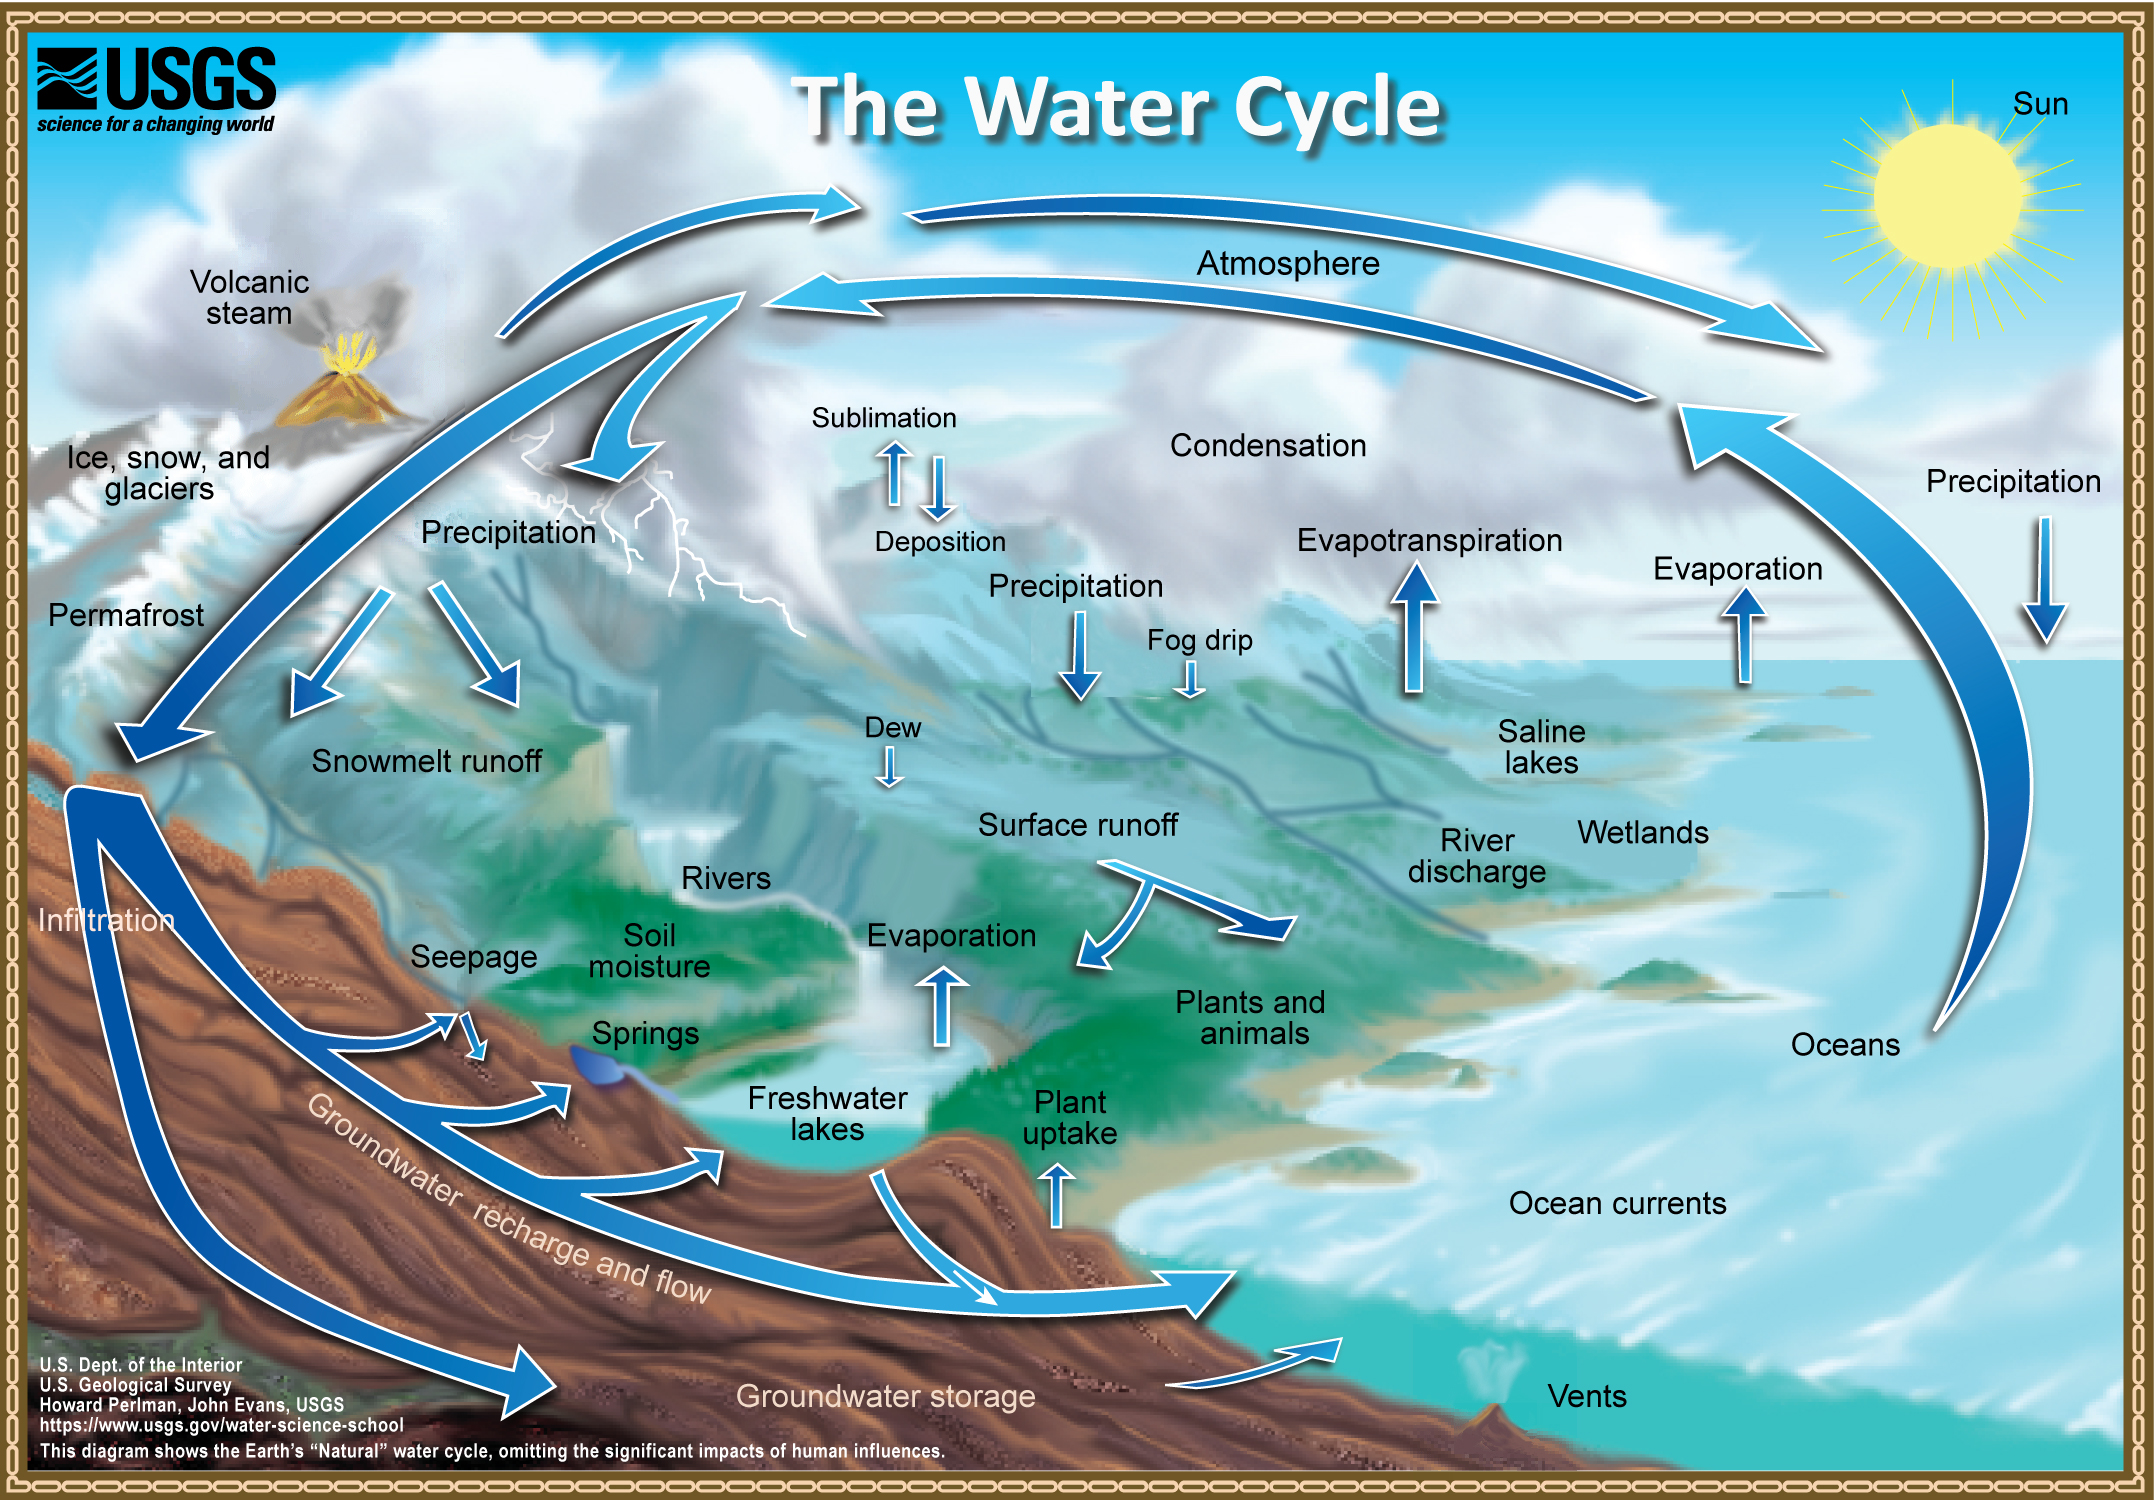
\includegraphics[width=0.7\textwidth]{water-cycle-natural} % Datei in "bilder/" bei LaTeX: eps, bei PDFLaTeX: jpg (o.ä.) 
	\caption{horologic cycle, \href{https://www.usgs.gov/media/images/water-cycle-natural-water-cycle}{source: https://www.usgs.gov/media/images/water-cycle-natural-water-cycle}} 
	\label{fig:hydrologic cycle}
\end{figure}\\
\section{Observation from Satellite Gravimetry}
However, it was extremely difficult to measure the global water storage change consistently. In some way. Remote sensing with satellite is the perfect tool for hydrology research, which has the ability to provide the data globally in a long term.\\\\
The GRACE twin satellites, launched 17 March 2002, are making detailed measurements of Earth's gravity field, which are caused by monthly changes in mass. The mass changes can be thought of as concentrated in a very thin layer of water thickness changes near the Earth's surface by moving ocean, atmospheric and land ice masses and by mass exchanges between these Earth system compartments. \\\\
There are 2 satellites with tandem polar orbit. Since the orbit is around the pole and the earth rotates itself, the satellites were able to get the whole view of the earth. Unlike the normal remote sensors, the GRACE satellites measured the gravity field of the earth. When the 2 satellites went over a mass anomaly like a big mountain, the distance of them will be a little bit smaller. By calculating this distance difference with the help of GPS system, the gravity filed of the earth along with the total water storage are able to be plotted monthly. 
\begin{figure}[htbp]
	\centering
	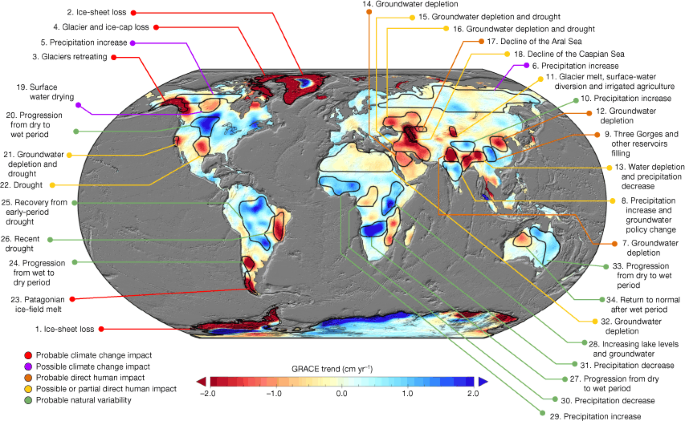
\includegraphics[width=0.6\textwidth]{TWSA} % Datei in "bilder/" bei LaTeX: eps, bei PDFLaTeX: jpg (o.ä.) 
	\caption{Water Storage Change} 
	\label{fig:TWSA}
\end{figure}
\begin{figure}[ht]
	\centering
	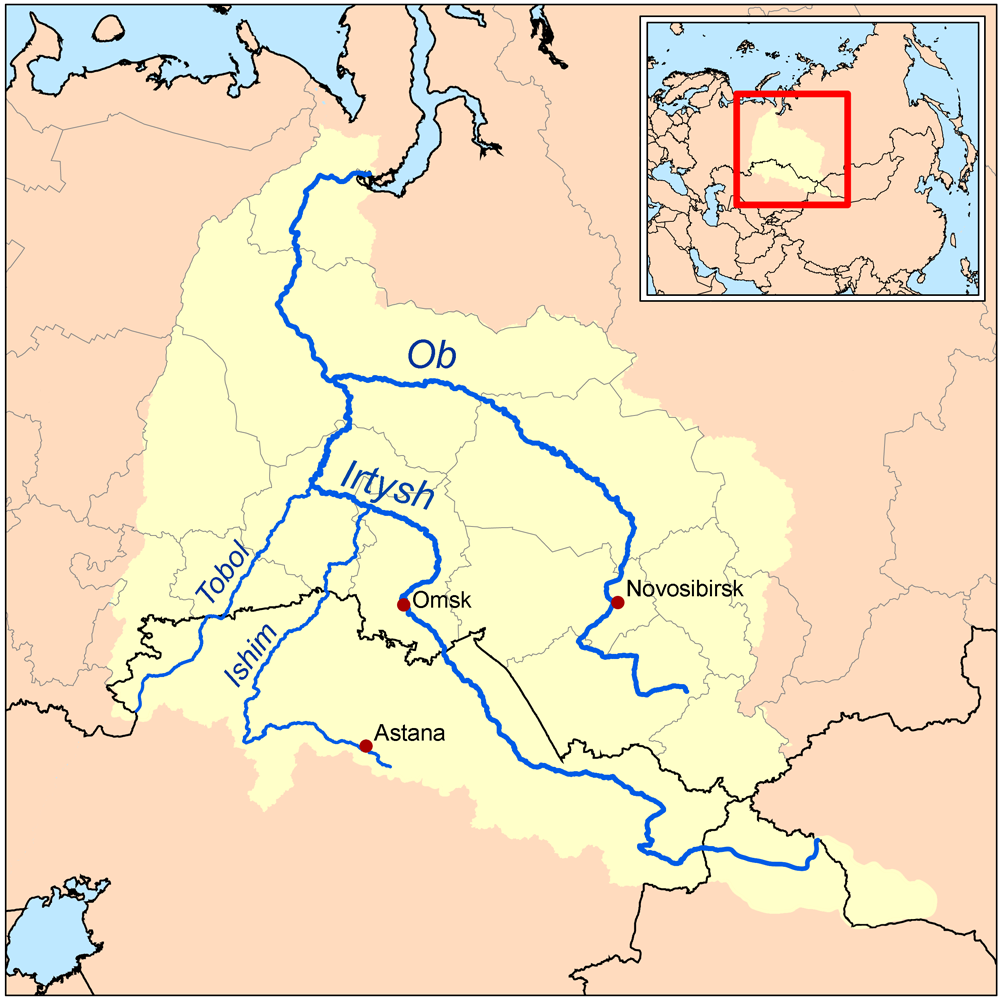
\includegraphics[width=0.6\textwidth]{Obbasin} % Datei in "bilder/" bei LaTeX: eps, bei PDFLaTeX: jpg (o.ä.) 
	\caption{Ob basin} 
	\label{fig:Obbasin}
\end{figure}\\
\section{Motivation}
Since 2002 it has been discovered that the water storage of many big basins has increased (see figure \ref{fig:TWSA}). One important basin of them is Ob basin in west Siberia (see figure \ref{fig:Obbasin}). The reason and the start time of this positive trend would be very interesting and also important. \\\\
The Thesis is organized in the following way:
\begin{itemize}
	\item Chapter 2 will describe the basic information of the study area, including the location, topography and climate.
	\item In chapter 3, the theoretical basis, the data source and the analyzing methods will be presented.
	\item The chapter 4 provides the results: the main reason of the main reason of the positiv trend would be critical discussed.
	\item In the last chapter, a brief summary and conclustion will be provided
\end{itemize}
\section{Objectives}